%
% experiment.tex -- Bild zum Thema Optische Fouriertransformation <opt>
%
% (c) 2023 Marco Niederberger, Yanick Schoch; OST Ostschweizer Fachhochschule
%

\documentclass[tikz]{standalone}
\usepackage{times}
\usepackage{txfonts}
\usepackage{pgfplots}

\pgfplotsset{compat=1.16}
\def\skala{1}

\begin{document}

\begin{tikzpicture}[>=latex,thick,scale=\skala]
    \draw[draw=none](-7,0)--(7,0);
    \node[inner sep=0pt, anchor=west] at (-7,0) {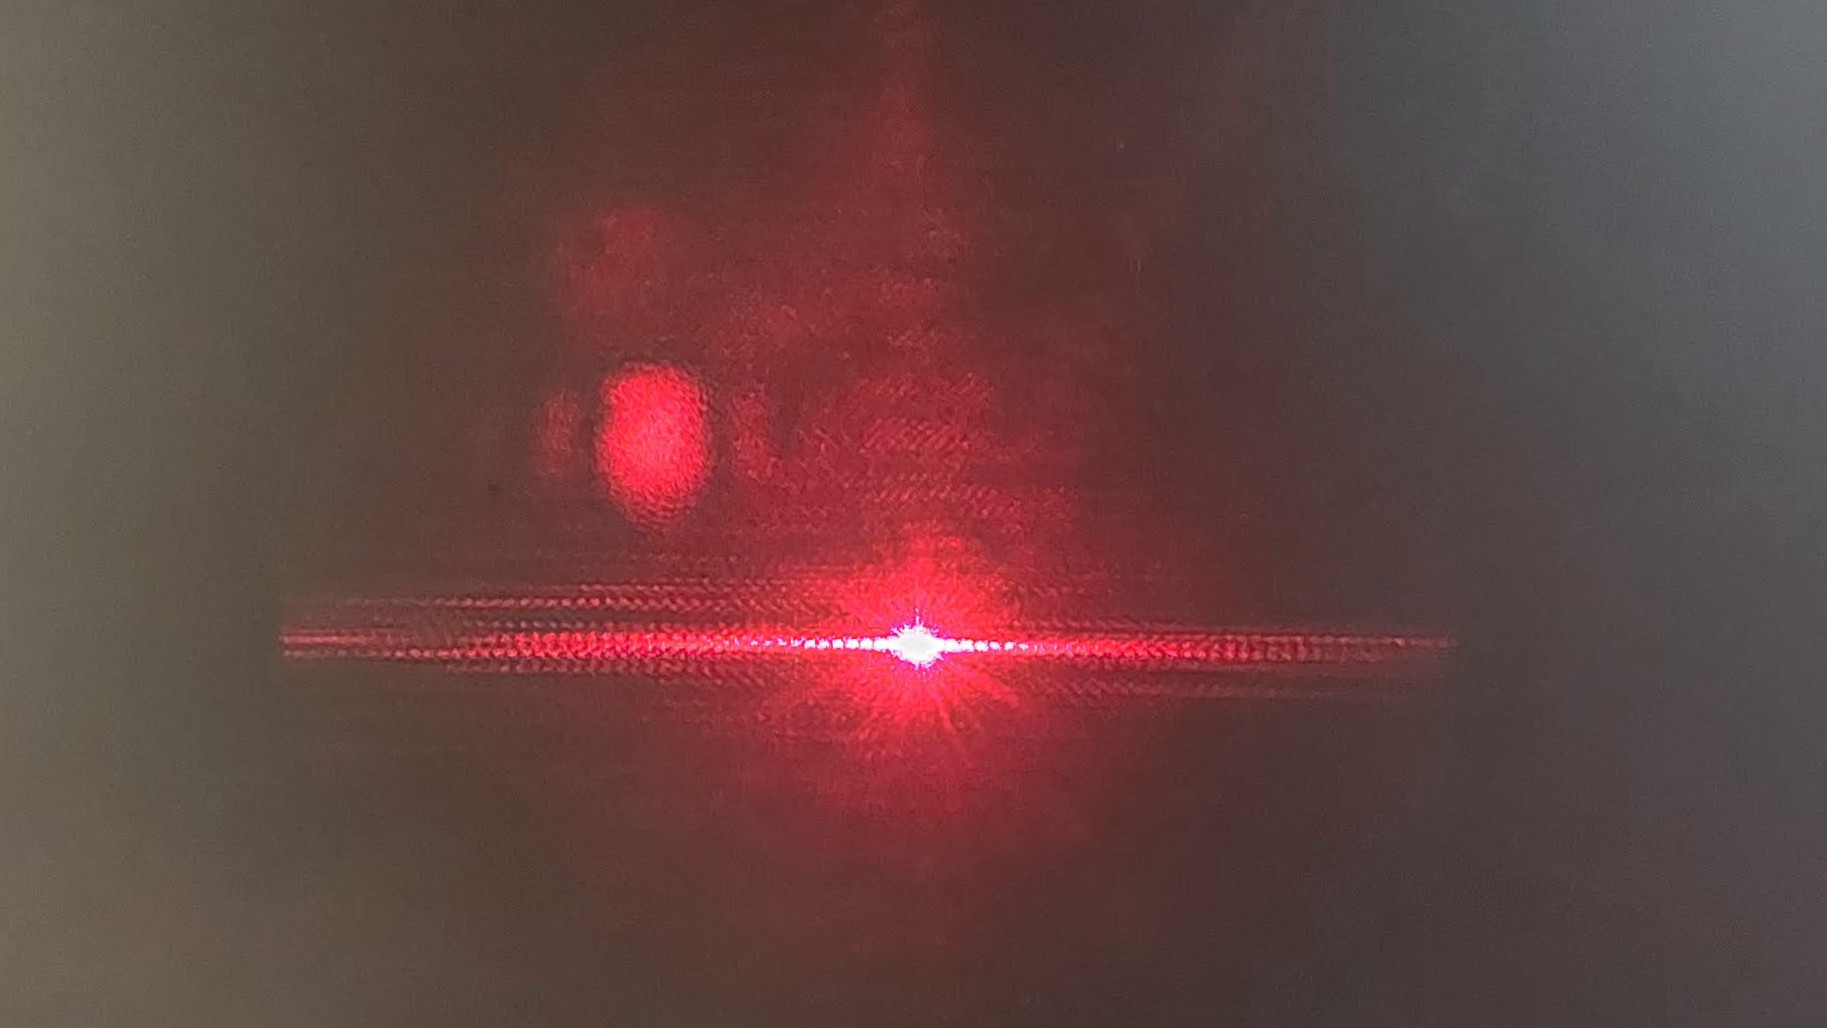
\includegraphics[width=60mm]{three_slit_spectrum.jpg}};
    \node[inner sep=0pt, anchor=east] at (7,0) {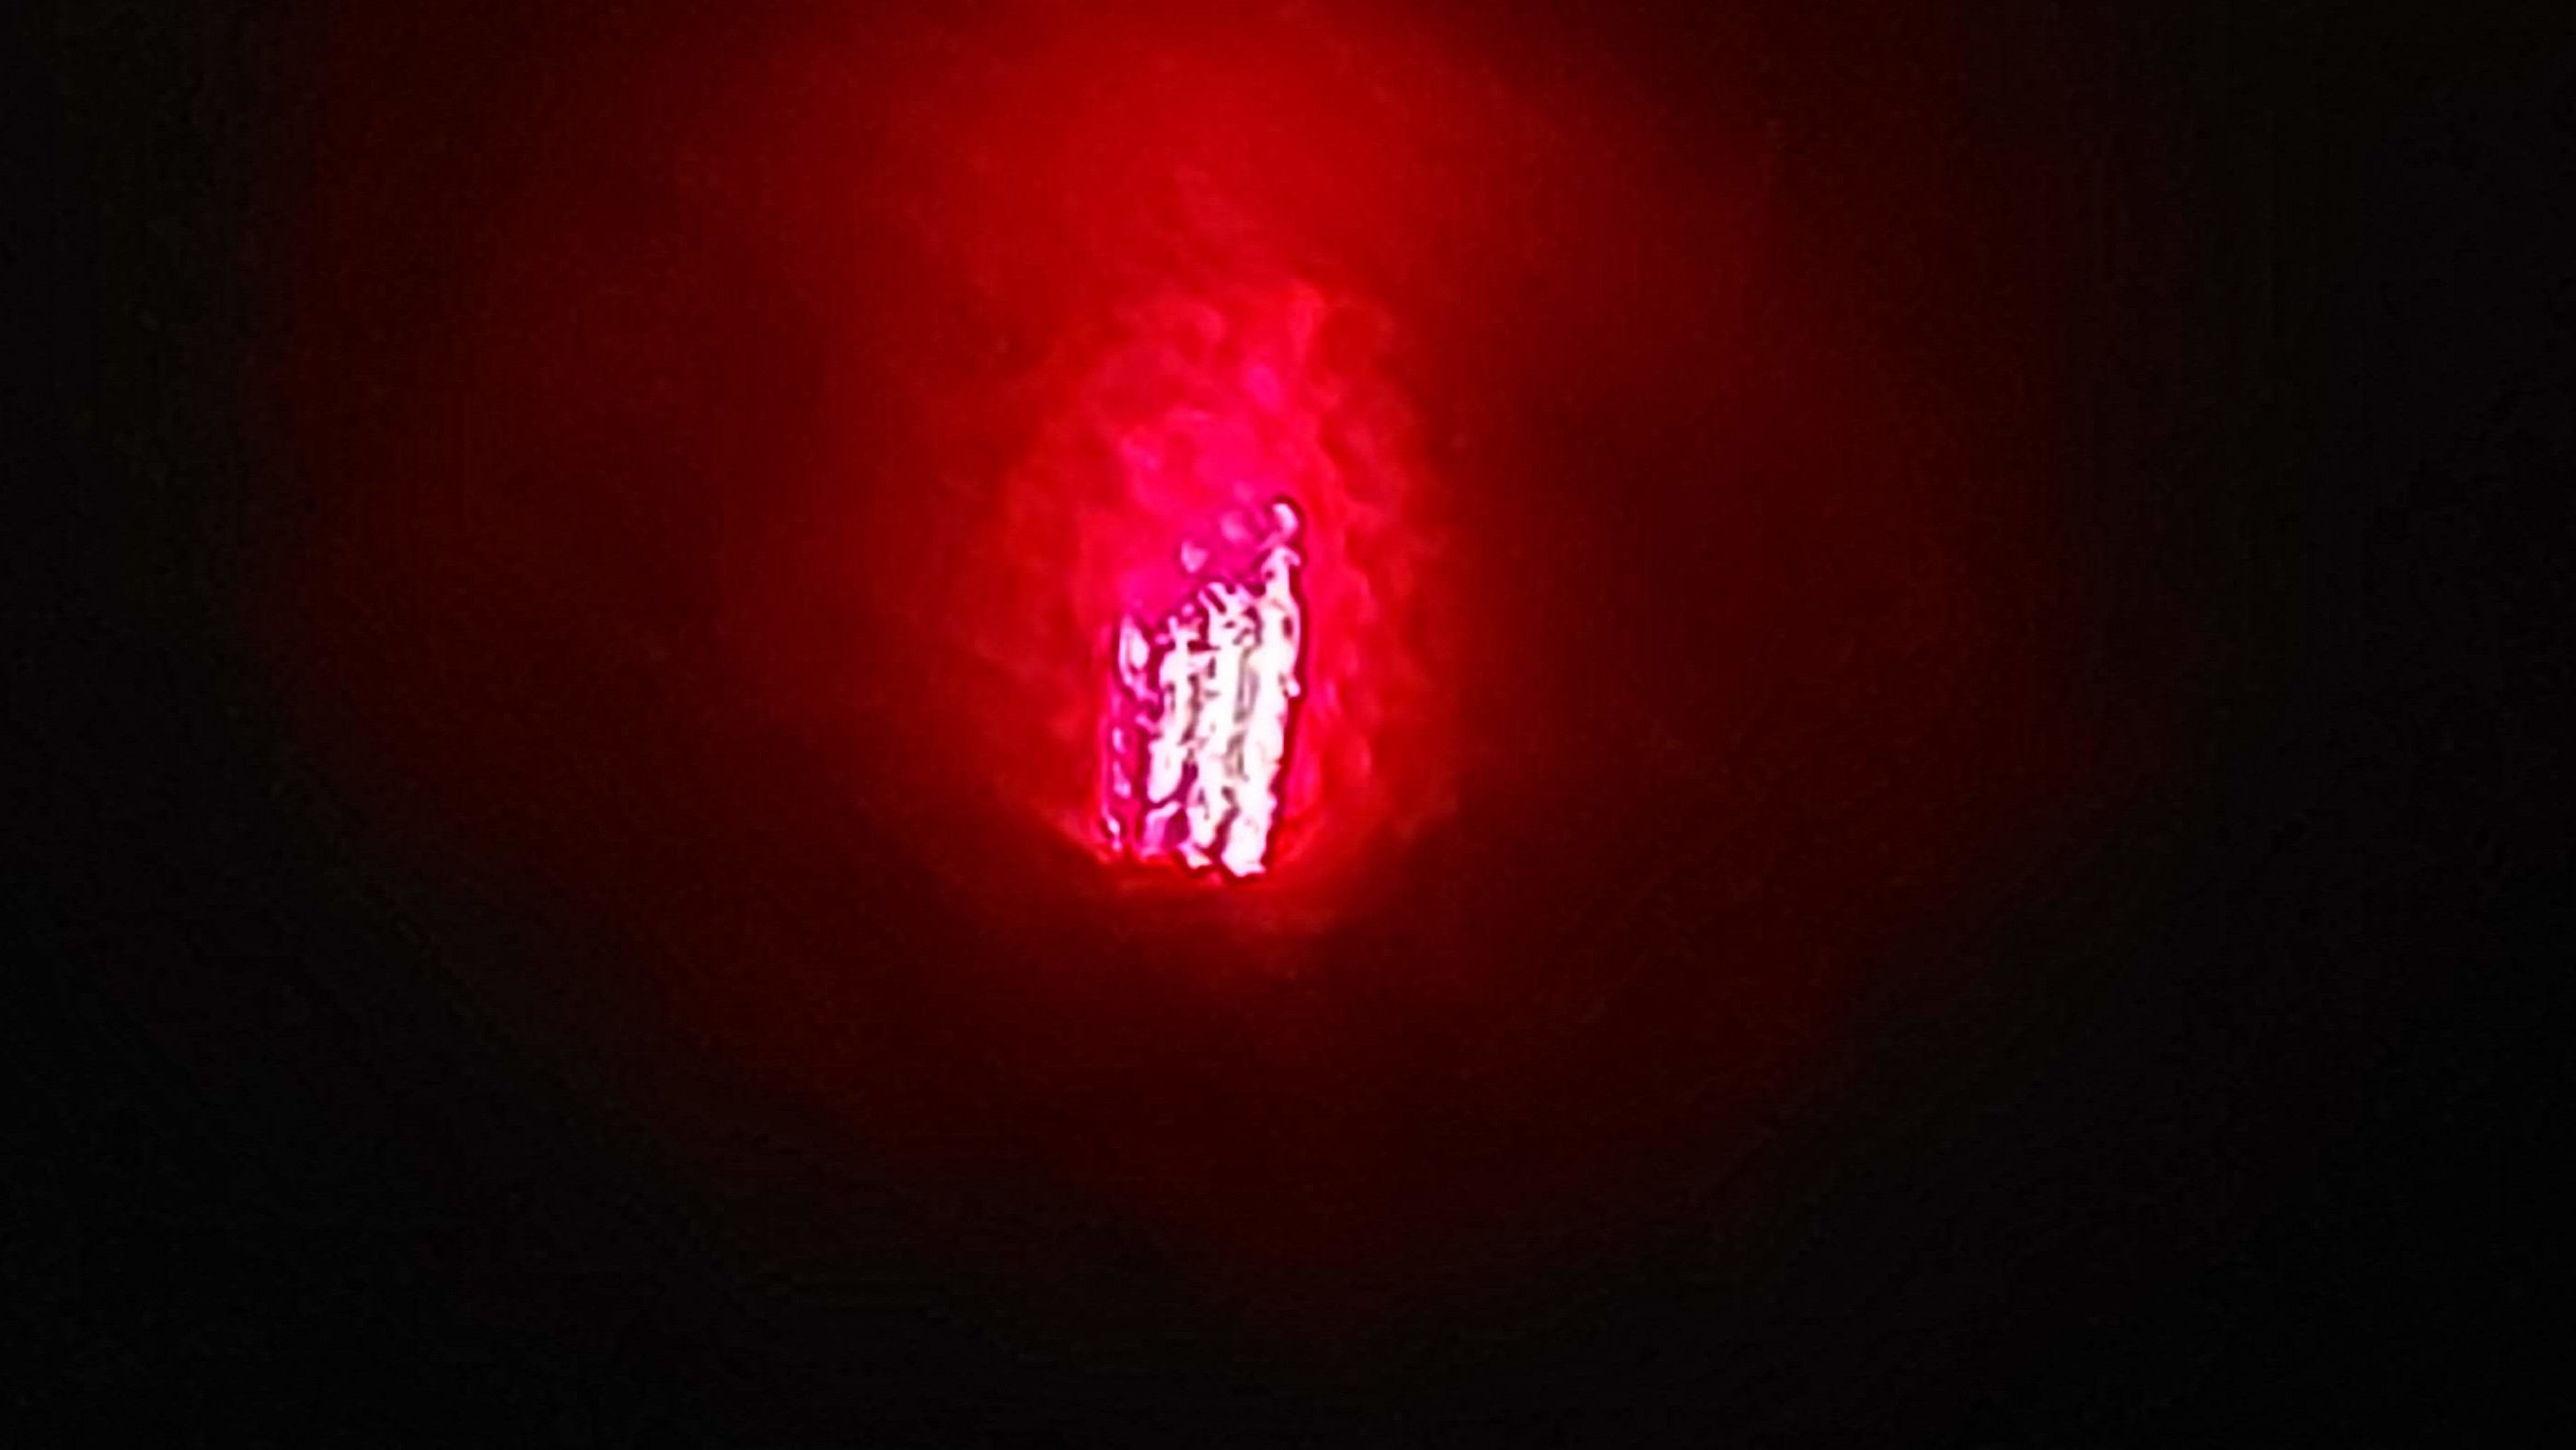
\includegraphics[width=60mm]{three_slit_back.jpg}};

    \node[draw=none] at (-4, -2.2) {a) Spektrum};
    \node[draw=none] at (4, -2.2) {b) Rücktransformation};

\end{tikzpicture}
\end{document}
